
Un content repository este un sistem de gestiune a informatiei, reprezentand o modalitate de stocare ierarhica a continutului ce furnizeaza suport atat pentru continut structurat cat si nestructurat, pentru cautare full text, versionare, tranzactii etc.


\bigskip

Arhiva de date RODA va trebui sa gestioneze informatii provenite din diverse surse, in formate diverse, inclusiv nestructurate. Din acest motiv, un punct important al sistemului informatic este reprezentat de integrarea si utilizarea unui sistem de gestiune de tip content repository. 


\bigskip

Tehnologia Apache Jackrabbit este o implementare a API-ului Java Content Repository (JCR -- specificat in cadrul normelor JSR 170 si 283).


\bigskip

Arhitectura generala a lui Jackrabbit poate fi descrisa pe 3 niveluri:

\begin{itemize}
\item nivelul de aplicatii referitoare la continut (Content application)
\item nivelul API
\item nivelul de implementare a depozitului de continut (Content repository implementation)
\end{itemize}

\bigskip

Arhitectura produsului Jackrabbit este descrisa in figura urmatoare:

\bigskip

\begin{center}
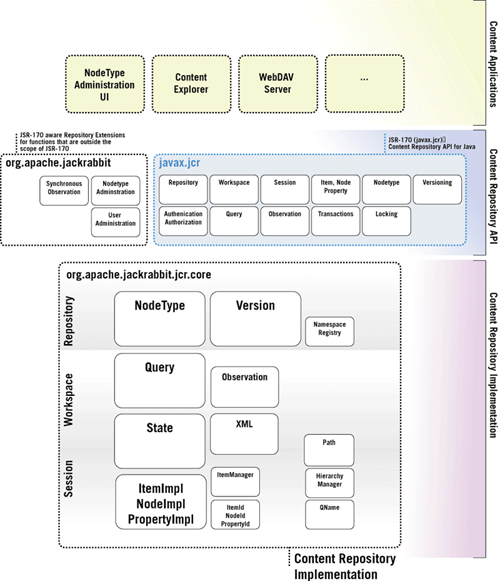
\includegraphics[width=4.5866in,height=5.3299in]{jackrabbit-img/jackrabbit-img001.png}
\end{center}

\bigskip

Componenta Content application interactioneaza prin intermediul API-ului din norma JSR-170 cu componenta Content repository implementation. Exista numeroase aplicatii care sunt disponibile pentru repository{}-urile JSR-170; unele dintre acestea sunt foarte generice (de exemplu, server-ul WebDAV), iar altele pot fi foarte specifice si pot utiliza un content repository pentru a stoca informatia utilizata in cadrul aplicatiilor respective. De exemplu, aplicatiile Java pot utiliza un content repository pentru a inlocui fisierele de proprietati, fisierele de configurare XML, anumite parti ale functionalitatii bazei de date, fisierele sistemului de operare, obiectele BLOB etc. Utilizarea unui content repository permite aplicatiei sa opereze cu un spatiu ierarhic de dimensiuni mari intr-o maniera scalabila, profitand automat de serviciile furnizate de content repository: versionare, interogare, tranzactii sau spatii de nume (namespaces). 

\bigskip

O aplicatie generica de tip content utilizeaza functionalitatile referitoare la tipurile nodurilor, controlul accesului si alte functionalitati pentru afisarea unei interfete utilizator \ sau a unui protocol de retea catre utilizatorul final, in mod independent de continutul care este stocat in repository. O aplicatie specifica de tip content presupune ca exista anumite tipuri de noduri asupra carora opereaza. De obicei, aceste tipuri de noduri sunt definite de catre aplicatie si sunt livrate impreuna cu aceasta. Aceste aplicatii utilizeaza un content repository care joaca rolul nivelului de persistenta, ca alternativa si evolutie a utilizarii unui sistem de gestiune a bazelor de date relationale sau a sistemului de fisiere.

\bigskip

Nivelul API se imparte in doua sectiuni principale:

\begin{itemize}
\item API-ul Content repository definit in JSR 170
\item un numar de caracteristici ale unui content repository care au fost retrase din specificatia JSR-170 deoarece sunt dificil de implementat in limbaje diferite de Java. \ \ \ 
\end{itemize}

\bigskip

In figura anterioara, portiunea din arhitectura corespunzatoare implementarii unui content repository reflecta componentele majore ale acestei implementari. Se poate observa ca, in cadrul unui content repository, exista 3 domenii (scope): repository, workspace, session. Functiile care opereaza asupra repository{}-ului pot fi asociate cel putin unui domeniu.


\bigskip

O componenta interna a lui Jackrabbit este managerul de persistenta (persistence manager - PM), care gestioneaza stocarea persistenta a nodurilor si proprietatilor. Fiecare workspace al unui content repository Jackrabbit utilizeaza un manager de persistenta separat care asigura stocarea continutului in workspace-ul respectiv. De asemenea, componenta care se ocupa de gestiunea versiunilor utilizeaza un manager de persistenta diferit. Managerul de persistenta apartine nivelului de baza al arhitecturii sistemului Jackrabbit, integritatea si performanta acestuia fiind de o importanta deosebita pentru stabilitatea si performanta intregului repository. 

In practica, un manager de persistenta este orice clasa Java care implementeaza interfata PersistenceManager. De asemenea, Jackrabbit contine un set de clase manager de persistenta predefinite, care acopera majoritatea necesitatilor de deployment. \ 


\bigskip

O alta componenta interna a acestei tehnologii este sistemul de fisiere (file system -- FS). Acesta implementeaza operatiile standard asupra fisierelor sistemului , in cadrul unui mecanism de stocare, care poate fi un sistem de fisiere normal, o baza de date, un server Webdav. O componenta de tip sistem de fisiere este orice clasa Java care implementeaza interfata FileSystem. Sistemele de fisiere sunt utilizate in Jackrabbit atat ca subcomponente ale managerilor de persistenta, cat si pentru nevoile generale de stocare (de exemplu, pentru stocarea indecsilor pentru cautarile full text). \ 


\bigskip

Gestiunea controlului accesului se poate realiza cu ajutorul pachetului javax.jcr.security, conform specificatiei JCR. Acesta acopera partea de autorizare, dar nu si gestiunea utilizatorilor, care constituie o caracteristica specifica implementarii Jackrabbit. Permisiunile (privilegiile) definite in JCR sunt urmatoarele:

\begin{itemize}
\item jcr:read -- privilegiul de a regasi in nod si de a obtine proprietatile sale si valorile acestora
\item jcr:modifyProperties -- privilegiul de a crea, sterge sau modifica valorile proprietatilor unui nod
\item jcr:addChildNodes -- privilegiul de a crea noduri copil ale unui nod
\item jcr:removeNode -- privilegiul de a sterge un nod
\item jcr:removeChildNodes -- privilegiul de a sterge nodurile copil ale unui nod
\item jcr:write: privilegiu agregat, ce contine jcr:read, jcr:modifyProperties, jcr:addChildNodes, jcr:removeNode, jcr:removeChildNodes
\item jcr:all -- privilegiu agregat, ce contine toate permisiunile posibile.
\end{itemize}

\bigskip

Specificatia JCR are in vedere listele de control al accesului (acl) bazate pe resurse. Aceasta presupue ca o resursa (adica, un nod) este asociata unei liste de intrari de tip accept/refuz pentru anumiti utilizatori sau grupuri. Un concept important al acl-urilor bazate pe resurse este ca acestea mostenesc acl-urile nodului parinte.

Acl-urile bazate pe resurse sunt stocate pentru fiecare resursa intr-un nod special, rep:policy. Acesta detine o lista de noduri copil rep:GrantACE (de obicei denumite allow, allow0 etc.) pentru intrarile ce corespund acordarii accesului si rep:DenyACE (de obicei denumite deny, deny0 etc.) pentru intrarile ce corespund refuzului accesului. 


\bigskip

Urmatorul fragment de cod constituie un exemplu de acordare a tuturor drepturilor catre toti utilizatorii, utilizand API-ul JCR:


\bigskip

AccessControlManager aMgr = session.getAccessControlManager();


\bigskip

// crearea unui set de privilegii ce contine jcr:all

Privilege[] privileges = new Privilege[] \{ aMgr.privilegeFromName(Privilege.JCR\_ALL) \};

AccessControlList acl;

try \{

\ \ \ \ // obtinerea primei politici aplicabile (pentru nodurile fara o astfel de politica definita)

\ \ \ \ acl = aMgr.getApplicablePolicies(path).nextAccessControlPolicy();

\} catch (NoSuchElementException e) \{

\ \ \ \ // nodul deja are o politica

\ \ \ \ acl = aMgr.getPolicies(path)[0];

\}

// stergerea intrarilor existente

for (AccessControlEntry e : acl.getAccessControlEntries()) \{

\ \ \ \ acl.removeAccessControlEntry(e);

\}

// adaugarea unei intrari noi pentru grupul ``everyone''

acl.addAccessControlEntry(EveryonePrincipal.getInstance(), privileges);


\bigskip

// resetarea politicii

aMgr.setPolicy(path, acl);


\bigskip

// salvarea sesiunii

session.save();


\bigskip

O alta abordare pentru specificarea si stocarea ACL-urilor este reprezentata de atribuirea catre anumiti utilizatori sau grupuri (principals) a unei liste de noduri asupra carora le este permis, sau nu, sa lucreze. Pentru a putea lucra cu ACL-uri de tip principal-based este necesara o extensie proprie Jackrabbit a API-ului pentru gestiunea controlului accesului.

O lista de control al accesului (rep:ACL) este stocata pentru fiecre utilizator sau grup. Aceasta lista consta din intrari de tip rep:GrantACE si rep:DenyACE.

Urmatorul fragment de cod exemplifica utilizarea ACL-urilor principal-based pentru controlul accesului in Jackrabbit.


\bigskip

JackrabbitSession js = (JackrabbitSession) session;


\bigskip

PrincipalManager pMgr = js.getPrincipalManager();

Principal principal = pMgr.getPrincipal(session.getUserID());


\bigskip

User user = ((User) js.getUserManager().getAuthorizable(session.getUserID()));

Principal principal = user.getPrincipal();


\bigskip

// Jackrabbit access control manager

JackrabbitAccessControlManager acMgr = (JackrabbitAccessControlManager) session.getAccessControlManager();


\bigskip

JackrabbitAccessControlPolicy[] ps = acMgr.getPolicies(principal); // or getApplicablePolicies()

JackrabbitAccessControlList list = (JackrabbitAccessControlList) ps[0];


\bigskip

JackrabbitAccessControlEntry[] entries = (JackrabbitAccessControlEntry[]) list.getAccessControlEntries();

JackrabbitAccessControlEntry entry = entries[0];


\bigskip

list.removeAccessControlEntry(entry);


\bigskip

// adaugarea unei intrari

Privilege[] privileges = new Privileges[] \{ acMgr.privilegeFromName(Privilege.JCR\_READ) \};

Map{\textless}String, Value{\textgreater} restrictions = new HashMap{\textless}String, Value{\textgreater}();

ValueFactory vf = session.getValueFactory();

restrictions.put({\textquotedbl}rep:nodePath{\textquotedbl}, vf.createValue({\textquotedbl}/some/path{\textquotedbl}, PropertyType.PATH));

restrictions.put({\textquotedbl}rep:glob{\textquotedbl}, vf.createValue({\textquotedbl}*{\textquotedbl}));

list.addEntry(principal, privileges, true /* allow or deny */, restrictions);


\bigskip

// reordonarea intrarilor

list.orderBefore(entry, entry2);


\bigskip

// resetarea politicii si salvare

acMgr.setPolicy(list.getPath(), list);

session.save();


\bigskip

API-ul pentru securitate utilizeaza Java Principals, ca mijloc de abstractizare, si nu presupune ca utilizatorii sunt stocati in JCR cu ajutorul modulului de gestiune a utilizatorilor din Jackrabbit. Un exemplu il constituie utilizatorii externi furnizati de catre un LoginModule via LDAP.


\bigskip

O caracteristica importanta a Jackrabbit consta in posibilitatea de a gestiona versiuni. Dintre ooeratiile posibile, amintim: check-in, check-out, obtinerea istoricului versiunilor, aplicarea unor etichete. Ulterior, pot fi adaugate functionalitati mai avansate, precum compararea versiunilor, inlocuire, revenire etc. Fiecare obiect versionat trebuie sa fie mapat intr-in nod JCR mix:versionable. \ 


\bigskip

Urmatorul fragment de cod regaseste istoricul versiunilor unui obiect study1:


\bigskip

VersionIterator versionIterator = ocm.getAllVersions({\textquotedbl}/study1{\textquotedbl});

while (versionIterator.hasNext())

\{

\ \ \ \ Version version = (Version) versionIterator.next();

\ \ \ \ System.out.println({\textquotedbl}version found : {\textquotedbl}+ version.getName() + {\textquotedbl} - {\textquotedbl} +

\ \ \ \ \ \ \ \ \ \ \ version.getPath() + {\textquotedbl} - {\textquotedbl} + \ version.getCreated().getTime());

\}

